\documentclass[11pt]{amsart}

\usepackage[utf8]{inputenc}
\usepackage{amsmath}
\usepackage{physics}
\usepackage{graphicx}

\renewcommand{\thesubsection}{\thesection.\alph{subsection}}

\title[Problem Set 4]{Semiconductors and Metals\\
			\hrulefill \small{ FYS3410: Problem Set 4 } \hrulefill}

\author{Candidate 33}

\date{\today}

\begin{document}

\maketitle

\setcounter{section}{2}

\section{Gallium Arsenide Semiconductor}
Gallium arsenide (GaAs) is a semiconductor with a direct band gap of $~1.42eV$ at room temperature. The experimental values for effective masses (in unit of free electron mass) are: $0.067$, $0.082$ and $0.45$ for electrons in the conduction band as well as light and heavy holes at the of the valence bands, respectively. 

The band structure of some semiconductors, including GaAs, around the point $\Gamma$ can be approximated by
\begin{equation}
E(\vb{k}) = E_0 + \frac{\hbar^2}{2m^*}(\vb{k}^2 - \Gamma) = C + Ak^2,
\end{equation}
where $m^*$ is the effective mass, and the factor $A$ is the curvature of the band. Setting $C=E_0=0$ one gets
\begin{equation}
A = \frac{\hbar^2}{2m^*}.
\end{equation}
Inserting for the different effective masser of the electrons and holes yields
\begin{align*}
A_1(m^* = \ \  0.067m_0) &= \ \ 0.569eVnm^2 \\ 
A_2(m^* = -0.082m_0) &= -0.465eVnm^2 \\
A_3(m^* = -0.450m_0) &= -0.085eVnm^2.
\end{align*}

\begin{figure}
\centering
	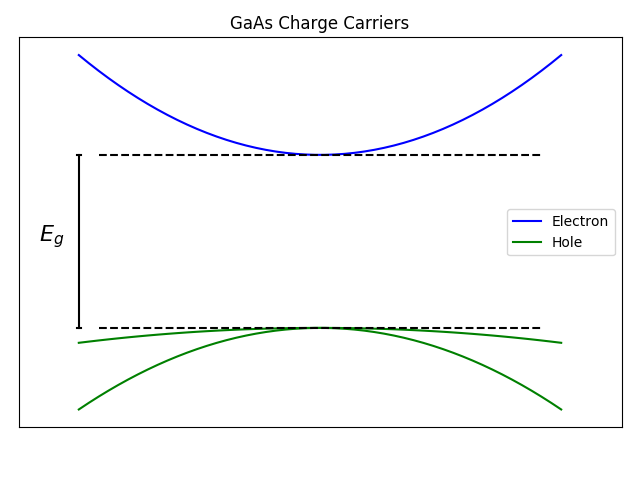
\includegraphics[width=0.75\textwidth]{problem3.png}
	\caption{Band gap in the vicinity of $\Gamma$ point. The effective mass of the holes (valence band) and electrons (conduction band) can be determined from the curvature of the graphs.}
	\label{fig:problem3}
\end{figure}

Figure \ref{fig:problem3} shows the band gap in the vicinity of $\Gamma$. The curvature of the energy level in $k$-space gives an indication to how heavy the hole or electron is. A steep curve gives light holes/electrons and a more moderate curvature means that the hole/electron is heavy.

\section{Hydrogen-like Dopants}
Phosphorous donors in a semiconductor consisting of pure silicone (Si) can be studied using a hyrogen-like model and effective mass approximation.

\subsection{Ionosation level of atoms} The ionisation energy of atomic Hydrogen is
\begin{equation}
E_0 = -\frac{e^4m}{2(4\pi\epsilon_0 \hbar)^2}
\end{equation}
as derived by Niels H. D. Bohr. In a semiconductor, such as Si, with dielectric constant $\epsilon$ we replace $e^2$ by $e^2/\epsilon$ and $m$ by effective mass $m^*$ to obtain
\begin{equation}
\label{eq:ionisationE}
E_d = \frac{e^4m^*}{2(4\pi\epsilon\epsilon_0 \hbar)^2}
\end{equation}
as the donor ionisation energy of the semiconductor. An atom of phosphorous (P) in a Si crystal can be approximated as a hydrogen-like atom, because P has one valence electron more than Si. Inserting the effective mass for electrons, $m^*\approx 0.2m$, and the permittivity, $\epsilon = 11.7$, for a Si crytal in equation \ref{eq:ionisationE}, we get
\begin{equation*}
E_d \approx 20meV
\end{equation*}

\subsection{Bohr Radius and Doping Concentration}
The Bohr radius of hydrogen is
\begin{equation}
a = \frac{4\pi\epsilon_0\hbar^2}{me^2}.
\end{equation}
By the same procedure as above, the Bohr radius of a donor is
\begin{equation}
a_d = \frac{4\pi\epsilon\epsilon_0\hbar^2}{m^*e^2}.
\end{equation}
Inserting for the permittivity and effective mass using Hydrogen approximation, as above, the bohr radius of P in Silicone becomes
\begin{equation*}
a_d \approx 3.1nm.
\end{equation*}

For the states to be localised and contained, there must at least be a distance $d=2a_d$ between each atom of P. This translates to a volume of $V_d = \frac{4}{3}\pi a_d^3$ per atom of P in the Si crystal. 

With appreciable orbit overlap, an ``impurity band'' is formed from the donor states. In theory, the Si crystal should transition to a metal state at zero temperature if the concentration of P gets to high. A metal-insulator transition has come to denote situations where the electrical conductivity of a material changes from a metal to insulator as a function of some external parameter.

For a sample of one cubic centimeter of Si, the maximum number of P donor atoms is
\begin{equation*}
\frac{(1\times10^{-2}m)^3}{\frac{4}{3}\pi(3.1\times10^{-9}m)^3} \approx 8 \times 10^{18}.
\end{equation*}
The observed metal transition of Si as donors of P are added is in reality at a bit lower concentration; just before $4\times10^{18} Pcm^{-3}$. See figure \ref{fig:rosenbaum1}\footnote{After T.F. Rosenbaum et al (1983).}.

\begin{figure}
\centering
	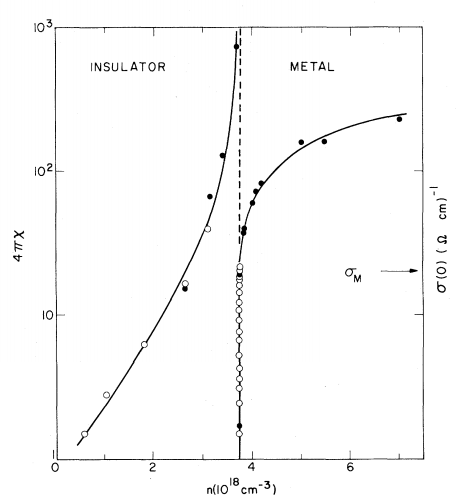
\includegraphics[width = 0.7\textwidth]{rosenbaum1.png}
	\caption{Semilog plot of oberved zero temperature susceptibility and conductivity as a function of phosphorous donor density.}
	\label{fig:rosenbaum1}
\end{figure}

\section{Carrier Concentration}
Temperature should have an effect on the carrier concentration of a semiconductor such as a homogenously doped sample of silicone (Si). 

\subsection{Equilibrium concentration for holes and electrons}
For very low temperatures, the sampel would be dominated by donor electrons given by
\begin{equation}
n = N_C e^{-\frac{E_d}{k_B T}}.
\end{equation}
When the temperature gets high enough, all donor electrons will be excited to the conduction band and the carrier concentration becomes equal to the number of donors, so that $n=N_d$. As the temperature rises further, valence electrons will be excited to the conduction band, the carrier concentration will be governed by the following intrinsic semiconductor relation
\begin{equation}
n_i = N_C e^{-\frac{E_g}{2k_BT}}.
\end{equation}
There are two transition points at
\begin{align*}
N_d = N_Ce^{-\frac{E_d}{k_BT}} \text{ and } N_d = N_ie^{-\frac{E_g}{2k_BT}},
\end{align*}
when the donor goes from beeing frozen out to full activation, and then to intinsic behaviour.

\end{document}